\documentclass[12pt,a4paper]{article}
\usepackage[T1]{fontenc}
\usepackage[utf8]{inputenc}
\usepackage{lmodern,microtype}
\usepackage[a4paper,left=25mm,right=25mm,top=23mm,textheight=672pt]{geometry}
\usepackage{amsmath,amssymb,amsthm,bm,mathtools}
\usepackage{graphicx,booktabs,array,longtable}
\usepackage[round,authoryear]{natbib}
\usepackage{setspace}
\usepackage{hyperref,xurl}
\hypersetup{hidelinks,pdfauthor={Jian Hou, Tan Meng, Maozai Tian}}
\usepackage[font=normalsize,labelfont=bf]{caption}
\newtheorem{theorem}{Theorem}
\newtheorem{proposition}{Proposition}
\newtheorem{lemma}{Lemma}
\newtheorem{corollary}{Corollary}
\theoremstyle{definition}\newtheorem{assumption}{Assumption}
\newtheorem{remark}{Remark}
\DeclareMathOperator{\Var}{Var}\DeclareMathOperator{\Cov}{Cov}
\DeclareMathOperator{\tr}{tr}\DeclareMathOperator{\argmin}{arg\,min}\DeclareMathOperator{\argmax}{arg\,max}
\newcommand{\E}{\mathbb E}\newcommand{\PP}{\mathbb P}\newcommand{\R}{\mathbb R}\newcommand{\ind}{\mathbf 1}
\newcommand{\op}{\mathrm{op}}\newcommand{\sg}{\mathrm{G}}\newcommand{\se}{\mathrm{E}}
\newcommand{\sT}{\mathrm{T}}\newcommand{\Yset}{\mathcal Y}\newcommand{\Lset}{\Lambda}
\newcommand{\wh}{\widehat}\newcommand{\wt}{\widetilde}\newcommand{\norm}[1]{\left\lVert#1\right\rVert}
\newcommand{\inner}[2]{\langle #1,#2\rangle}\newcommand{\Pp}{\mathbb P_n}
\newcommand{\mc}{\mathrm{mc}}\newcommand{\parens}[1]{\left(#1\right)}
\setlength{\parindent}{1.25em}\setlength{\parskip}{0pt}
\setlength{\emergencystretch}{2em}
\graphicspath{{../figures/}}
\doublespacing

% Float placement preserves the body font and line spacing.
\renewcommand{\topfraction}{0.9}
\renewcommand{\bottomfraction}{0.8}
\renewcommand{\textfraction}{0.08}
\renewcommand{\floatpagefraction}{0.65}
\setcounter{topnumber}{3}
\setcounter{bottomnumber}{2}

\newenvironment{procedurebox}
{\begin{center}\begin{minipage}{0.94\textwidth}\hrule\vspace{0.6em}}
{\vspace{0.4em}\hrule\end{minipage}\end{center}}


\newcommand{\SimCovMin}{0.944}
\newcommand{\SimCovMax}{0.968}
\newcommand{\SimAlignedWidthMin}{0.731}
\newcommand{\SimAlignedWidthMax}{0.831}
\newcommand{\SimReversalWeight}{0.000}
\newcommand{\SimHarmMax}{0.000}
\newcommand{\EpaWidthMin}{0.746}
\newcommand{\EpaWidthMax}{1.000}
\newcommand{\EpaJointMin}{0.935}
\newcommand{\EpaJointMax}{0.970}
\newcommand{\NumAgreement}{1.000}
\newcommand{\NumCriticalError}{0.000}
\newcommand{\NumGainError}{0.000}
\newcommand{\NumCovError}{0.000}

\title{Surrogate-assisted local conditional distribution inference\\with certified simultaneous gains}
\author{Jian Hou\textsuperscript{a}, Tan Meng\textsuperscript{b}, and Maozai Tian\textsuperscript{b}\thanks{Corresponding author: mztian@ruc.edu.cn.}\\[.4em]
\normalsize\textsuperscript{a}College of Systems Engineering,\\
\normalsize National University of Defense Technology, Changsha 410073, China\\
\normalsize\textsuperscript{b}Center for Applied Statistics, School of Statistics,\\\normalsize Renmin University of China, Beijing 100872, China}
\date{}
\begin{document}
\begin{center}\setstretch{1.0}
{\Large\bfseries Surrogate-assisted local conditional distribution inference\par
with certified simultaneous gains\par}
\vspace{0.8em}
{\normalsize Jian Hou\textsuperscript{a}, Tan Meng\textsuperscript{b}, and Maozai Tian\textsuperscript{b}\par}
\vspace{0.4em}
\begin{minipage}{\textwidth}\centering\normalsize\setstretch{1.0}
\textsuperscript{a}College of Systems Engineering,\\
National University of Defense Technology, Changsha 410073, China\\[0.4em]
\textsuperscript{b}Center for Applied Statistics, School of Statistics,\\
Renmin University of China, Beijing 100872, China\\[0.4em]
Correspondence: mztian@ruc.edu.cn
\end{minipage}
\end{center}
\begin{abstract}\normalsize
Low-cost surrogates can improve inference from scarce reference measurements, but minimising average estimation variance need not shorten a simultaneous confidence band. We study this distinction for a local conditional distribution under selective verification. A common borrowing path joins a surrogate-free reference estimator to a surrogate-assisted estimator. We choose its weight by a lower confidence bound on the paired reduction in a Gaussian simultaneous critical value. The gain vanishes exactly at the reference estimator, and its covariance-estimation error decreases with the borrowing weight. This cancellation yields an anchor-adaptive oracle bound without a unique optimal weight. We develop an implementable multiplier calibration, independent numerical guards, and simultaneous inference after selection, including a dependence-valid aggregation of sample rotations. A local binary submodel identifies a reference-information scale for certifying weak improvements. Simulations compare average-variance, direct-band, projection and certified borrowing. An air-monitoring application separates historical mean calibration from subsequent distributional verification and measures the reference budget needed to recover humidity-specific exceedance discrepancies.
\end{abstract}
\noindent\textbf{Keywords:} Augmented estimation; Conditional distributions; Gaussian approximation; Negative transfer; Selective verification; Simultaneous inference.
\section{Introduction}
In many modern applications, the quantity of scientific interest is expensive to measure, while a cheap surrogate is available for nearly every unit. Cheapness does not settle the inferential question, because a surrogate that predicts well on average can be inaccurate in the neighbourhood or in the tail where inference is required. In the air-monitoring study below, a linear calibration trained on historical collocations leaves a mean difference of $-0.191$ micrograms per cubic metre near 30\% relative humidity in the subsequent audit period, while the calibrated sensor assigns 6.068\% of local observations above a concentration of 15 against 9.307\% for the reference. Mean calibration therefore leaves the distributional question open: which of these discrepancies can be established from a limited reference sample.

We observe covariates $X$ and a surrogate $S$ for most units, a reference outcome $Y$ only in a verified subset, and we target the conditional distribution of $Y$ at a chosen $x_0$. Augmented inverse-probability weighting remains valid when the fitted outcome regression is inaccurate, and it joins a surrogate-free anchor to a surrogate-assisted estimator through a common borrowing path. The question we ask is which feature of uncertainty should determine the weight on that path.

For a simultaneous band, average variance is the wrong criterion. The band's critical value depends on the joint covariance across thresholds, including how the correction redistributes variance. Proposition~\ref{prop:separation} gives a valid two-threshold path whose population trace-minimising weight reduces total variance and increases the simultaneous critical value, so an exactly known optimal average-variance weight can lengthen the band. Estimating a band-optimal weight adds a second difficulty, because a small apparent reduction may be sampling noise in the covariance estimate.

The observed-data representation is classical. Surrogate-outcome and two-phase methods establish it \citep{Pepe1992,RobinsRotnitzkyZhao1994,TaoZengLin2017,Tsiatis2006}, rejective two-phase designs quantify its efficiency gains \citep{YangDing2025}, and combining probability with non-probability samples extends it to modern data sources \citep{YangKimSong2021}. Semi-supervised inference supplies the complementary lesson that unlabelled units can sharpen inference for prediction performance and regression parameters \citep{GronsbellCai2018,GronsbellEtAl2022,AzrielEtAl2022,ChakraborttyCai2018,ZhangBrownCai2019,Song2024}, and modern learning with missing covariates shows when such gains persist under flexible estimators \citep{MaWangSamworth2026}. Adaptive augmentation optimises auxiliary-information use for parameter estimation \citep{CaoTsiatisDavidian2009}. These procedures choose auxiliary information for parameters, and the selection criterion for a threshold-indexed local distribution has remained open.

Prediction-powered inference has made the label-scarce setting a central object of study. Its basic construction and efficient variants \citep{AngelopoulosEtAl2023,AngelopoulosDuchiZrnic2023,ZrnicCandes2024} treat a fitted predictor as an auxiliary variable, and follow-up work examines label contamination, surrogate-powered regularisation, adaptive shrinkage and post-prediction inference \citep{SesiaEtAl2025,JiLeiZrnic2025,ChenEtAl2025,LiIgnatiadis2025,MiaoEtAl2025}. The finite-reference cost of estimating borrowing weights is now documented \citep{mani2025nofreelunch,Eyre2025}, and \citet{KallusMao2025} characterise the efficiency gain from surrogates in estimation with limited outcome data. These results certify or regularise a fitted predictor for scalar targets; a weight chosen for a simultaneous band on a whole conditional distribution requires a different criterion.

Distributional targets have their own line of work. \citet{SuiEtAl2026} study prediction-powered conditional functionals, \citet{TestaEtAl2025} allow selective labels with decreasing overlap, and \citet{Wang2026} develops surrogate-assisted distributional inference for transported outcomes. Local distribution estimation with fully observed outcomes is established \citep{CattaneoJanssonMa2024,CattaneoEtAl2024}, conformal methods deliver distribution-free prediction sets for counterfactuals, individual effects and survival times \citep{LeiCandes2021,CandesLeiRen2023}, and generation-powered and multi-source extensions develop functional borrowing and confidence-region volume \citep{zhang2026generation,li2026multisource}. Rearrangement handles crossing quantiles \citep{ChernozhukovEtAl2010}. Anderson's covariance-dominating operator improves Gaussian probabilities of centred convex symmetric sets \citep{Anderson1955}, and a fitted path need not admit such an ordering.

Guarantee calibration, selection control and transfer complete the picture. Local weights and randomization trade bias for localised validity in conformal prediction \citep{HoreBarber2025}, conditional and selection-conditional coverage are characterised with matching impossibility results \citep{GibbsEtAl2025,JinRen2025}, and prediction sets adapt to unknown covariate shift through doubly robust calibration \citep{QiuEtAl2023,YangEtAl2024}. Error-controlled selection with subsampling \citep{ShahSamworth2013} and covariate-powered testing \citep{IgnatiadisHuber2021} control the selection error itself, while doubly robust testing with generative models inserts learned components into test statistics \citep{ZhangEtAl2026}. Transfer theory quantifies when auxiliary data help and when they harm, in high-dimensional and nonparametric regression and classification \citep{LiCaiLi2022,GuHanDuan2025,AuddyEtAl2026}. Our negative-transfer question is local: a surrogate correction can help the anchor at some thresholds and hurt it at others.

We evaluate the resulting procedure in two settings. A simulation study compares six borrowing criteria under alignment, weak surrogates, local reversal, absent signal and an exact zero path, then isolates the contribution of pairing in a matched ablation, tests dense threshold grids and non-Gaussian outcomes, and evaluates exact operating characteristics in a binary local experiment. An air-monitoring application separates historical mean calibration from subsequent distributional verification: all 2019 site-days fit and freeze the calibration and the candidate regressions, and designed Bernoulli verification on the 2020--2021 audit frame measures which humidity-specific exceedance discrepancies a given reference budget can establish.
We develop \emph{paired gain certification} for a local distribution. We estimate the difference between the anchor and candidate simultaneous critical values under a common covariance, and its uncertainty vanishes at zero borrowing. We exploit that cancellation to obtain an oracle bound proportional to the beneficial borrowing weight, an implementable multiplier calibration with independent numerical guards, and simultaneous inference after selection without a unique optimal weight. A binary local experiment gives the reference-information scale for certifying weak improvements. The general learning-and-testing principle is established \citep{angelopoulos2021learn}; the contribution here is the paired critical-value geometry, its local information scaling, and its use in distributional inference.

Section~2 defines the estimator and algorithm, Section~3 states the certification, inference and information results, Section~4 compares borrowing criteria and evaluates their extensions, and Section~5 applies the method to dated air-monitoring collocations before the concluding discussion.


\section{Local estimation and paired borrowing}
In this section we define the reference target, the augmentation path and the certified borrowing rule. We work conditionally on an independent training sample and treat the verification probability as known; Section~S8 covers estimated probabilities.

\subsection{The reference distribution and augmentation path}
We observe $O=(W,R,RY)$, where $W$ includes $X$ and $S$. Assume $R\perp Y\mid W$ and initially treat $\pi(W)=p e(W)$ as known, with $e$ bounded above and away from zero. Let $Z_y=\ind(Y\leq y)$. For a bounded nonnegative kernel $K_h(X-x_0)=K\{(X-x_0)/h\}$, put
\begin{equation}\label{eq:target}
 \mu_h=\E K_h,\quad v_h=h^d,\quad f_h=\mu_h/v_h,\quad
 F_h(y)=\frac{\E(K_hZ_y)}{\mu_h}.
\end{equation}
Equation~\eqref{eq:target} defines the inferential target at the declared resolution $h$. The point target $F_0(y\mid x_0)$ additionally requires localisation-bias control.

We use an independent training sample that produces bounded candidate distribution functions $q_y(X)$ and $m_y(W)$. The anchor omits the surrogate from its outcome regression. Define $D_y=m_y-q_y$ and $a_{\lambda,y}=q_y+\lambda D_y$, $0\leq\lambda\leq1$. The augmented signal has the linear representation
\begin{equation}\label{eq:signal}
 U_{\lambda,y}=q_y+\frac R\pi(Z_y-q_y)
       +\lambda\left(1-\frac R\pi\right)D_y
       =U_{0,y}+\lambda B_y.
\end{equation}
Equation~\eqref{eq:signal} shows that the correction enters linearly and that, conditional on the training sample, $\E(U_{\lambda,y}\mid W)=\E(Z_y\mid W)$ and $\E(B_y\mid W)=0$. Candidate accuracy changes covariance, not the target.

On a threshold grid $\Yset_J=\{y_1,\ldots,y_J\}$, form
\begin{equation}\label{eq:psi}
 \Psi=\sqrt{p/v_h}\,K_h
       \binom{U_0-F_h}{B},\qquad
 \Omega=\E(\Psi\Psi^\top),\qquad H_\lambda=(I_J,\lambda I_J).
\end{equation}
Equation~\eqref{eq:psi} stacks the anchor score and the correction, and the covariance path is quadratic:
\begin{equation}\label{eq:path}
 \Sigma_\lambda=H_\lambda\Omega H_\lambda^\top
 =\Omega_{00}+\lambda(\Omega_{01}+\Omega_{10})+\lambda^2\Omega_{11}.
\end{equation}
For the evaluation sample $\se$, the kernel ratio admits the exact representation derived in Section~S3, and $\wh f_{h,\se}=\PP_{\se}K_h/v_h$; a zero denominator gives the full $[0,1]$ distribution band.

\subsection{The uncertainty criterion}
For $G_\lambda\sim N(0,\Sigma_\lambda)$, let
\begin{equation}\label{eq:gain}
 c_\Omega(\lambda)=\operatorname{Quantile}_{1-\alpha}\norm{G_\lambda}_\infty,
 \qquad g_\Omega(\lambda)=c_\Omega(0)-c_\Omega(\lambda).
\end{equation}
Equation~\eqref{eq:gain} defines the object of the selector: the reduction in the Gaussian simultaneous critical value at the same resolution, sample size and confidence level. A fixed positive band shape is allowed by rescaling both score blocks before forming $\Omega$; the shape is common to all weights. The trace rule minimises $\tr(\Sigma_\lambda)$ instead.

\begin{proposition}[Separation of the criteria]\label{prop:separation}
There is a valid distributional augmentation path for which the trace minimiser $25/41$ reduces $\tr(\Sigma_\lambda)$ from $0.340$ to $0.318$, but increases its 95\% simultaneous critical value from $0.983562$ to $0.996761$.
\end{proposition}
The construction takes $S\sim\operatorname{Bernoulli}(0.2)$, with $Y\mid S=0$ uniform on $\{1,2\}$ and $Y\mid S=1$ uniform on $\{0,2\}$. At thresholds $(0,1)$, use $q=(0.1,0.5)$, $m(S)=\{0.5S,0.5+0.4(S-0.2)\}$ and independent verification with $p=0.1$. Figure~\ref{fig:separation} displays the two criteria. The proof uses marginal Gaussian probability inequalities, not the accuracy of a numerical optimiser.

\begin{figure}[htbp]\centering
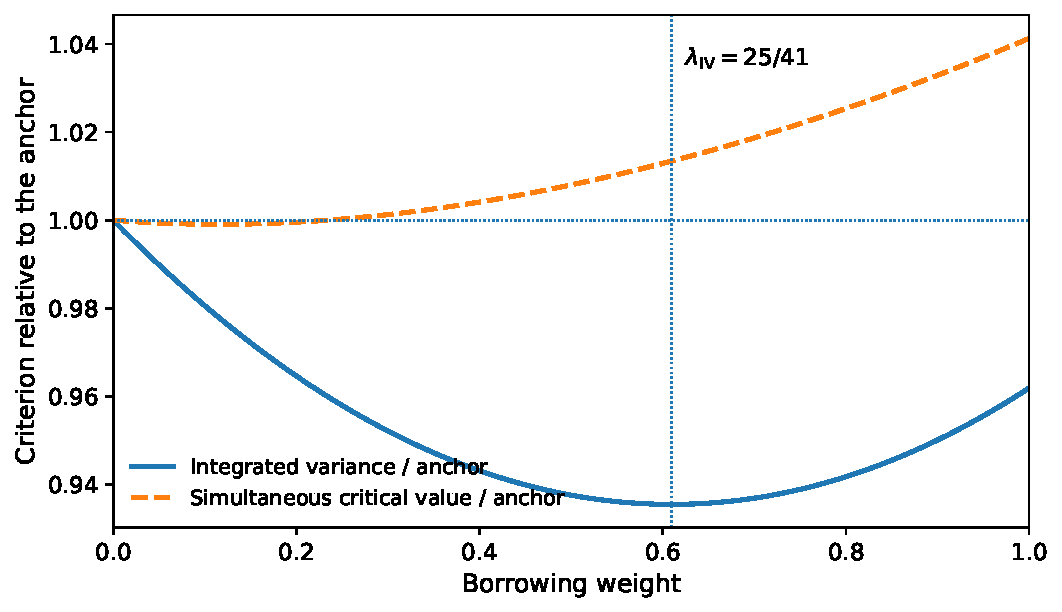
\includegraphics[width=.82\linewidth]{figure1_separation.pdf}
\caption{The exact two-threshold example separates the trace and simultaneous-band criteria. Both curves are relative to Anchor; at the trace optimum $25/41$, the simultaneous critical value exceeds the anchor value. These are Gaussian calculations, not Monte Carlo estimates.}\label{fig:separation}
\noindent Alt text: The trace improves while the simultaneous criterion worsens at the trace optimum.
\end{figure}


\subsection{An implementable paired calibration}
We now replace the covariance set by a sample estimate. A second, independent sample $\sg$ estimates $\Omega$. We write $\wh F=\PP_{\sg}K_hU_0/\PP_{\sg}K_h$, $\wh r_i=(U_{0,i}-\wh F,B_i)^\top$ and
\begin{equation}\label{eq:moments}
 \wh\Omega=\frac p{v_h}\PP_{\sg}(K_h^2\wh r\wh r^\top),\quad
 \wh A=\frac p{v_h}\PP_{\sg}(K_h^2\wh r),\quad
 \wh\ell_i=\frac{K_{h,i}(U_{0,i}-\wh F)}{\PP_{\sg}K_h}.
\end{equation}
Equation~\eqref{eq:moments} gives the plug-in moments on the gate sample. The covariance influence contribution is
\begin{equation}\label{eq:covif}
 \wh C_i=\wh\Psi_i\wh\Psi_i^\top-\wh\Omega
       -E_0\wh\ell_i\wh A^\top-\wh A\wh\ell_i^\top E_0^\top,
       \qquad E_0=\binom{I_J}{0}.
\end{equation}
The last two terms in \eqref{eq:covif} account for estimating the anchor centring; omitting them changes the covariance uncertainty being calibrated.

Let $\Lset$ be a finite weight grid containing zero. For $\lambda>0$, define
\begin{equation}\label{eq:gradient}
 D_\lambda(\Omega)=\nabla_\Omega\{g_\Omega(\lambda)/\lambda\},\qquad
 \wh s_{i\lambda}=\inner{D_\lambda(\wh\Omega)}{\wh C_i}.
\end{equation}
We centre these scores across observations. Independent standard normal multipliers $\xi_i$ approximate
$\max\{0,\max_{\lambda>0}n_{\sg}^{-1}\sum_i\xi_i\wh s_{i\lambda}\}$.
Let $\wh t_\delta$ be an upper simulated quantile at probability $1-\delta$. We add a nonnegative second-order cushion $b_N$ and use fresh Gaussian draws to obtain simultaneous numerical intervals $[\underline c_\lambda,\overline c_\lambda]$ for the plug-in critical values. Note that the lower interval at the anchor is exactly the anchor critical value. We set
\begin{equation}\label{eq:rule}
 \wh L(0)=0,\quad
 \wh L(\lambda)=\underline c_0-\overline c_\lambda
                       -\frac{\wh t_\delta+b_N}{\sqrt{n_{\sg}}}\,\lambda
                       \quad(\lambda>0),\qquad
 \wh\lambda\in\argmax_{\lambda\in\Lset}\wh L(\lambda).
\end{equation}
Equation~\eqref{eq:rule} is the selection rule used throughout: a weight is adopted only when its certified lower bound on the gain is positive.

\begin{procedurebox}
\textbf{Algorithm 1: Certified local simultaneous inference}
\begin{enumerate}
\item Fix $x_0$, $h$, the threshold grid $\Yset_J$, the weight grid $\Lset$, the three roles and the error budgets $(0.049,0.0005,0.0005)$.
\item Fit the anchor $q$ and the candidate $m$ on the fitting role.
\item On the gate role, compute $\wh\Omega$, $\wh A$, the centred scores $\wh s_{i\lambda}$ and the multiplier quantile $\wh t_\delta$; form the numerical intervals $[\underline c_\lambda,\overline c_\lambda]$.
\item Select $\wh\lambda$ by \eqref{eq:rule}.
\item On the evaluation role, form $\wh F_{\se,\wh\lambda}$ and the simultaneous band with the calibrated critical value.
\item Rotate the three roles and aggregate the evaluation estimates.
\end{enumerate}
\end{procedurebox}



\section{Certification and simultaneous inference}
\subsection{A covariance-set benchmark and paired sensitivity}
Condition throughout on the training sample. Let $\mathcal C_G$ be a nonempty compact set of positive semidefinite joint covariance matrices with conditional coverage at least $1-\delta$. An ideal paired lower bound and its selector are
\begin{equation}\label{eq:ideal}
 L_G(\lambda)=\inf_{Q\in\mathcal C_G}\{c_Q(0)-c_Q(\lambda)\},\qquad
 \lambda_G\in\argmax_{\lambda\in\Lset}L_G(\lambda).
\end{equation}
Both critical values inside the braces use the same $Q$, so $L_G(0)=0$ exactly, and the benchmark separates the statistical certificate from its numerical approximation.

\begin{theorem}[Paired certification]\label{th:ideal}
Let $\lambda^\star\in\argmax_{\lambda\in\Lset}g_\Omega(\lambda)$. Then
$\Pr\{g_\Omega(\lambda_G)<0\mid\sT\}\leq\delta$. On $\{\Omega\in\mathcal C_G\}$,
\begin{equation}\label{eq:genericregret}
 0\leq c_\Omega(\lambda_G)-c_\Omega(\lambda^\star)
 \leq\sup_{Q\in\mathcal C_G}|g_Q(\lambda^\star)-g_\Omega(\lambda^\star)|.
\end{equation}
Neither uniqueness nor curvature of the minimiser is required.
\end{theorem}
Indeed, $g_\Omega(\lambda_G)\geq L_G(\lambda_G)\geq L_G(\lambda^\star)$ and $L_G(\lambda_G)\geq0$; the substantive issue is the size of the paired covariance perturbation.

\begin{theorem}[Anchor-adaptive sensitivity]\label{th:sensitivity}
Fix $J$, $\alpha$, $\kappa>0$ and $B<\infty$. Suppose $Q,Q'$ belong to
$\mathcal K_{\kappa,B}=\{Q\succeq0:\norm Q_\op\leq B,
H_\lambda QH_\lambda^\top\succeq\kappa I_J,\ 0\leq\lambda\leq1\}$.
There is a finite $C=C(J,\alpha,\kappa,B)$ such that
\begin{equation}\label{eq:pairedlip}
 |g_Q(\lambda)-g_{Q'}(\lambda)|\leq C\lambda\norm{Q-Q'}_\op.
\end{equation}
If $\mathcal C_G\subset\mathcal K_{\kappa,B}$ has radius $\varepsilon_G$ about a common centre, the right side of \eqref{eq:genericregret} is at most $2C\lambda^\star\varepsilon_G$.
\end{theorem}
The proof differentiates the Gaussian rectangle quantile twice with respect to its covariance and uses the cancellation at $\lambda=0$. The joint matrix may be singular, and only its output covariance needs to be positive definite, so an exactly zero correction is allowed. Constants depend on dimension and conditioning, and a growing grid requires the explicit dimension-dependent conditions in the Supplement.

\subsection{Feasible calibration under scarce verification}
Write $N_G=n_Gph^d$ and $N_E=n_Eph^d$. We impose the following conditions for the implemented procedure. The observations in each role are independent copies within a triangular row, the roles are disjoint, $\mu_h\asymp h^d$, the kernel and candidate functions are bounded, and $0<c_e\leq e\leq C_e<\infty$. Both local information indices diverge. For a fixed threshold and weight grid, output covariances stay in a compact positive definite set. Finally, the normalised nonzero covariance-influence scores satisfy the Lindeberg and covariance-consistency conditions stated in Supplementary Section~S3. These are conditions on the fitted path, and correct specification of either regression is unnecessary.

\begin{theorem}[Feasible paired calibration]\label{th:feasible}
Under these conditions, the covariance estimator in \eqref{eq:moments} has the influence expansion \eqref{eq:covif}, and
\begin{equation}\label{eq:slopelinear}
 \frac{g_{\wh\Omega}(\lambda)-g_\Omega(\lambda)}{\lambda}
   =\frac1{n_G}\sum_{i\in G}\inner{D_\lambda(\Omega)}{C_i}
     +O_P(N_G^{-1})
\end{equation}
uniformly over nonzero grid weights. Suppose $b_N\sqrt{N_G}\to0$ and $N_Gb_N\to\infty$, and the computed score gradients obey the consistency condition in Section~S3. If the numerical critical-value intervals fail jointly with probability at most $\eta_c$, and the simulated multiplier quantile fails as an upper quantile with probability at most $\eta_t$, then \eqref{eq:rule} satisfies
\begin{equation}\label{eq:asympsafety}
 \Pr\{g_\Omega(\wh\lambda)<0\mid\sT\}
       \leq\delta+\eta_c+\eta_t+o(1).
\end{equation}
There is an event $\mathcal A_N$ with conditional probability at least
$1-\delta-\eta_c-\eta_t-o(1)$ and a nonnegative $R_N=O_P(N_G^{-1/2})$ such that, on $\mathcal A_N$, every grid oracle $\lambda^\star$ satisfies
\begin{equation}\label{eq:feasible-regret}
 0\leq c_\Omega(\wh\lambda)-c_\Omega(\lambda^\star)
 \leq\lambda^\star(R_N+\wh t_\delta+b_N)+e_{\mc}(\lambda^\star).
\end{equation}
Here $\wh t_\delta=O_P(N_G^{-1/2})$, $e_{\mc}(\lambda)$ sums the anchor and candidate numerical interval widths, and $e_{\mc}(0)=0$. The bound retains the certificate's failure probability; at an anchor oracle its zero regret is asserted on $\mathcal A_N$.
\end{theorem}
Theorem~\ref{th:ideal} gives a finite-sample covariance-set statement and Theorem~\ref{th:feasible} an asymptotic multiplier statement. The software implements the latter, with exact finite-sample protection for the Monte Carlo quantile errors, and an observable Bernstein covariance ball for the benchmark is given in Section~S2. For $D=s_N\widetilde D$ with $s_N\to0$, the score statement applies after normalising by the nonzero path scale under the corresponding Lindeberg condition, and $D=0$ returns the anchor exactly.

\subsection{Coverage, whole distributions and rotating roles}
\begin{theorem}[Independent evaluation]\label{th:coverage}
Let $\mathcal L\subseteq[0,1]$ be a fixed finite set or the compact interval. Assume the evaluation score process admits a Gaussian approximation uniformly over $\lambda\in\mathcal L$, its covariance estimate is uniformly consistent, and its Gaussian maximum is uniformly continuous at the target quantiles. For any $\mathcal L$-valued weight measurable with respect to the training and selection samples, the independently calibrated grid band has coverage at least $1-\alpha-\eta_E-o(1)$, where $\eta_E$ bounds its Monte Carlo quantile error. No convergence to a unique deterministic weight is needed.
\end{theorem}
Conditional on training and selection, the chosen weight is fixed in \eqref{eq:identity}; uniform Gaussian approximation and covariance consistency give the conclusion. Under a uniformly bounded local score envelope, standard Gaussian rectangle bounds apply when $\log^7(n_EJ)/N_E\to0$ \citep{cck2016clt}, and continuous-index counterparts use the local increment and entropy conditions in Section~S4.

If grid limits $(l_j,u_j)$ cover $F_h(y_j)$, the envelopes
\begin{equation}\label{eq:envelope}
 l(y)=\max\{0,\max_{y_j\leq y}l_j\},\qquad
 u(y)=\min\{1,\min_{y_j\geq y}u_j\}
\end{equation}
cover the entire distribution, with empty maxima and minima interpreted as zero and one. Inverting these envelopes gives simultaneous quantile bounds even at atoms, at the price of resolution-dependent width. A second-order localisation bias is negligible for the point target when $\sqrt{N_E}h^2\to0$, and smooth positive density additionally gives the usual quantile-process derivative.

Rotating three roles is analysed by calibrating each role at error $\alpha/3$ and intersecting its whole-distribution bands; a union bound gives overall error at most $\alpha+o(1)$ without independence between the three bands. Conditioning on all three selected weights would instead reveal evaluation information. Convex combinations of their endpoints are also valid but can be wider, and Section~S5 gives both constructions.

\subsection{How much reference information certifies a gain?}
Consider $S\in\{-1,1\}$ equally likely and $Z=\ind(Y=0)$ with
$\Pr_\theta(Z=1\mid S)=1/2+\theta S$. Set $q=1/2$, $D=dS$, $0<d<1/4$, and verify independently with probability $p$. Then
\begin{equation}\label{eq:binary}
 p\Var_\theta(U_\lambda)=\tfrac14+(1-p)(d^2\lambda^2-2d\theta\lambda).
\end{equation}
For $0<\theta<d$, $\lambda^\star=\theta/d$ and the optimal critical-value gain is
$z_{1-\alpha/2}(1-p)\theta^2+O(\theta^4)$.

\begin{theorem}[Local certification boundary]\label{th:boundary}
If a positive-gain certificate is issued on an event $A$ with $\Pr_0(A)\leq\delta$, then
$\Pr_\theta(A)\leq\delta+\sqrt{2n_Gp}|\theta|$.
Localising the association to a box-kernel support of probability $r_h$ replaces $n_Gp$ by $n_Gpr_h$. Conversely, conditional on $k$ local verified observations,
\begin{equation}\label{eq:binarycert}
 \theta_L=\frac1{2k}\sum_{i=1}^k S_i(2Z_i-1)
        -\sqrt{\frac{\log(1/\delta)}{2k}},\qquad
 \wh\lambda=\min\{1,(\theta_L)_+/d\}
\end{equation}
has harmful-selection probability at most $\delta$, and selects a positive weight with probability at least $1-\beta$ if
$\theta\geq\sqrt{\log(1/\delta)/(2k)}+\sqrt{\log(1/\beta)/(2k)}$.
\end{theorem}
The proof bounds observed-data divergence by $4n_Gp\theta^2$ and applies a one-sided Hoeffding bound for the converse. In this submodel the signal boundary is $N_G^{-1/2}$ and the oracle-gain boundary is $N_G^{-1}$, so numerical error must be smaller than the gain to retain this resolution, and a finite weight mesh must resolve the local optimum.

\section{Simulation study}
\label{sec:simulation}
\subsection{Design, comparators and performance measures}
We separate three questions: whether borrowing improves distribution estimation, whether it shortens a simultaneous band, and whether the available reference information supports a positive-gain certificate. All methods use the same generated observations, verification indicators and role assignments within each replication. The primary experiment has twelve cells with 500 replications per cell; Supplementary Table~S1 retains the complete cell-by-method results, and Table~\ref{tab:simulation} compares all six methods at a common sample size and reference fraction. We generate independent $X\sim U[-1,1]$, $\varepsilon,\eta\sim N(0,1)$ and set
\[
 Y=\mu(X)+\sigma(X)\varepsilon,\quad
 \mu(x)=1.2x+0.6x^2,\quad \sigma(x)=0.8+0.25x^2,\quad
 S=\ell(X)Y+\tau\eta.
\]
Alignment uses $\ell(x)=1$ and $\tau=0.4$; the weak-surrogate design changes $\tau$ to 1.6. Local reversal sets $\ell(x)=-1$ for $|x|\leq0.4$ and $\ell(x)=1$ elsewhere. The no-signal design takes $\ell(x)=0$, whereas the zero-path design sets the fitted surrogate candidate exactly equal to the anchor, distinguishing an absent correction from a correction estimated from an uninformative surrogate.

The target is $F_h(\cdot\mid0)$ with an Epanechnikov kernel, $h=0.35$, and seven thresholds $0.8\Phi^{-1}(u_j)$, where the $u_j$ are equally spaced from 0.1 to 0.9. The weight grid is $\{0,0.1,\ldots,1\}$. We use sample sizes 6,000 and 12,000 with reference fractions 0.05, 0.10 and 0.20. Random verification is compared with bounded selective verification favouring larger standardised surrogate readings, whose exact probability is given in Section~S9. Three equal roles fit Gaussian location--scale regressions, select borrowing and evaluate the distribution. The anchor mean uses $(1,X,X^2)$ and the surrogate mean additionally uses $S$, so both global fits face the locally reversed relationship in the reversal experiment.

Anchor and Full fix $\lambda=0$ and 1. Trace minimises the estimated covariance trace; Plug-in minimises the estimated simultaneous critical value without a statistical gain penalty. Recall from \eqref{eq:path} that $\Omega_{11}$ is the correction block of the joint covariance: Projection uses a matrix control variate estimated from this block with ridge $0.05\tr(\wh\Omega_{11})/J$, and the matrix can mix threshold corrections and reverse their signs, so its candidate class is larger than the scalar path. Paired uses \eqref{eq:rule}. The statistical selection error is 0.049, the two numerical selection errors receive 0.0005 each, and evaluation allocates 0.049 to Gaussian coverage and 0.001 to numerical calibration. Radial gradients use 8,192 directions, gate calibration uses 3,999 multiplier draws, and critical-value protection uses 32,768 independent Gaussian draws.

We report simultaneous coverage, the within-replication band-width ratio to Anchor, selected weights and grid-integrated squared error,
\[
 \operatorname{ISE}_{J}=J^{-1}\sum_{j=1}^J
       \{\wh F_h(y_j)-F_h(y_j)\}^2,
\]
using the raw estimator on the inferential grid. Harmful selection is assessed from the population covariance of each fitted path, $c_\Omega(\wh\lambda)>c_\Omega(0)+10^{-4}$, which differs from larger realised squared error. Covariances and their Gaussian criteria are evaluated by deterministic quadrature. Standard errors for continuous summaries use independent replications, and coverage and harm frequencies have binomial intervals.

\subsection{Gains, reversal and the cost of certification}
We now report the gains and their cost. Across the twelve cells, Paired coverage ranges from \SimCovMin{} to \SimCovMax{}, and in aligned cells its mean width ratio is \SimAlignedWidthMin{}--\SimAlignedWidthMax{}. At $n=6,000$ and $p=0.10$ under random verification, grid ISE falls from $3.074\times10^{-3}$ for Anchor to $1.567\times10^{-3}$ for Paired at width ratio 0.747, while Full, Trace and Plug-in reach width ratios near 0.722 with grid ISE near $1.42\times10^{-3}$. Certification costs width relative to uncritical borrowing, and the cost declines with information. Paired's mean weight rises from 0.507 to 0.807 as $p$ grows from 0.05 to 0.20, its adoption probability rises from 0.862 to 1.000, and doubling the sample size at $p=0.10$ increases the mean weight from 0.718 to 0.822 while the width ratio falls from 0.747 to 0.731. Under selective verification at $p=0.05$ the adoption probability is 0.752 and the mean weight 0.421, so a nominal reference fraction may support different borrowing decisions under different designs.

We use the weak-surrogate cell to separate usefulness from certifiability. Full shortens bands to 0.954 of the anchor width with grid ISE $2.526\times10^{-3}$ against $2.899\times10^{-3}$, yet Paired chooses zero in all 500 replications because the gate cannot establish enough improvement under the stated confidence and numerical budgets. Weak-signal non-adoption therefore differs from absence of surrogate information.

Reversal shows the protection. Full increases mean width by 11.4\% and grid ISE from $3.080\times10^{-3}$ to $3.909\times10^{-3}$, with assessed harmful-selection frequency 0.994, while Paired returns Anchor and Trace and Plug-in select positive borrowing in only 0.6\% of replications. Projection behaves differently: its reversal width ratio is 0.805 with grid ISE $1.901\times10^{-3}$, because the unrestricted matrix can exploit the reversed relationship that the nonnegative scalar path rejects. The certificate controls selection along the proposed path, and this comparison marks its scope. Under no signal, Trace and Plug-in have harmful-selection frequencies 0.310 and 0.312 with mean Gaussian gains $-0.000217$ and $-0.000232$ and width ratios near 1.000, whereas Paired is never harmful; Projection has width ratio 1.013 and mean gain $-0.007431$. In the exact zero-path cell every method reduces to the anchor.

\begin{figure}[htbp]\centering
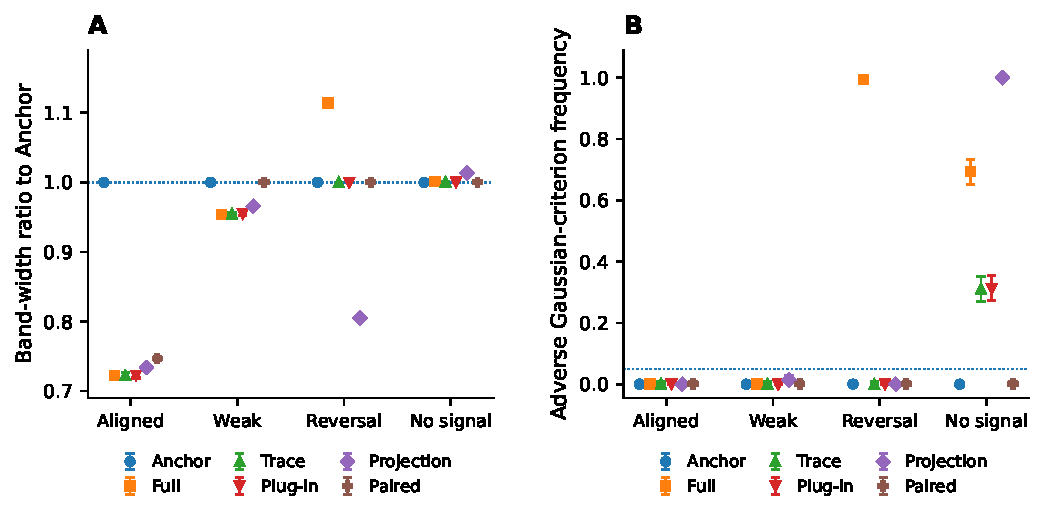
\includegraphics[width=\linewidth]{v2/figure2_simulation_comparison.pdf}
\caption{Six-method comparisons with $n=6,000$ and $p=0.10$ under random verification. (A) Mean within-replication band-width ratios; bars are $\pm1.96$ Monte Carlo standard errors. (B) Assessed harmful-selection frequencies, using critical-value tolerance $10^{-4}$; bars are exact binomial 95\% intervals. Each mechanism has 500 replications. The dotted reference in (B) is 0.05.}\label{fig:simulation_comparison}
\noindent Alt text: Projection benefits from reversal; Paired retains Anchor under weak and absent signals. Near-null harm frequencies can be high despite small width changes.
\end{figure}


\subsection{Pairing, dense thresholds and robustness}
We isolate the contribution of pairing with a matched ablation of six additional cells and 500 replications each. Unpaired constructs separate one-sided bounds for the anchor critical value and the candidate-critical-value maximum, with error control proved in Section~S3.5. Both selectors use the same fitted candidates, samples, weight mesh, numerical critical-value intervals and total $0.05$ selection-error budget; the distinction is statistical, since Unpaired adds two absolute-error bounds whereas Paired calibrates their difference and preserves its vanishing scale at the anchor. Under alignment at $p=0.05,0.10,0.20$, Paired's width ratios are 0.802, 0.747 and 0.769 against 1.000, 1.000 and 0.993 for Unpaired, with adoption probabilities 0.858, 0.998, 1.000 and 0.000, 0.000, 0.032. Both rules return the anchor under reversal and the no-signal correction. Paired coverage across the six cells is 0.928--0.958, with the weakest cell also showing low Anchor coverage; Section~S10 reports the exact binomial intervals and all six-method comparisons.

We test how far the mechanism extends in the remaining cells. We evaluate 21, 51 and 101 nested thresholds spanning probabilities $0.02$--$0.98$, under alignment and selective local reversal, with 200 datasets per mechanism shared across resolutions and a declared covariance enlargement $10^{-8}I_J$; Paired coverage ranges from 0.935 to 0.965, its aligned width ratios are 0.765, 0.782 and 0.798, and it retains the anchor under reversal. Monotone envelopes are evaluated on a common 1,001-point grid, so the continuum guarantee rests on the monotonicity result rather than on interpolation of seven simulated coordinates. We examine seven further cells, each with 300 replications: standardised $t_3$, skewed and mixture errors, a ten-category outcome, two-dimensional localisation, neighbour-distribution candidates and fitted logistic verification probabilities. The six known-design cells give Paired coverage 0.950--0.970 with width ratios 0.686--0.841, and the learned-probability sensitivity gives coverage 0.963 and width ratio 0.768 while requiring the nuisance-drift conditions in Section~S8. The complete conditional CDF, including ordinal cutpoints, is computed from each generating distribution.

\begin{figure}[htbp]\centering
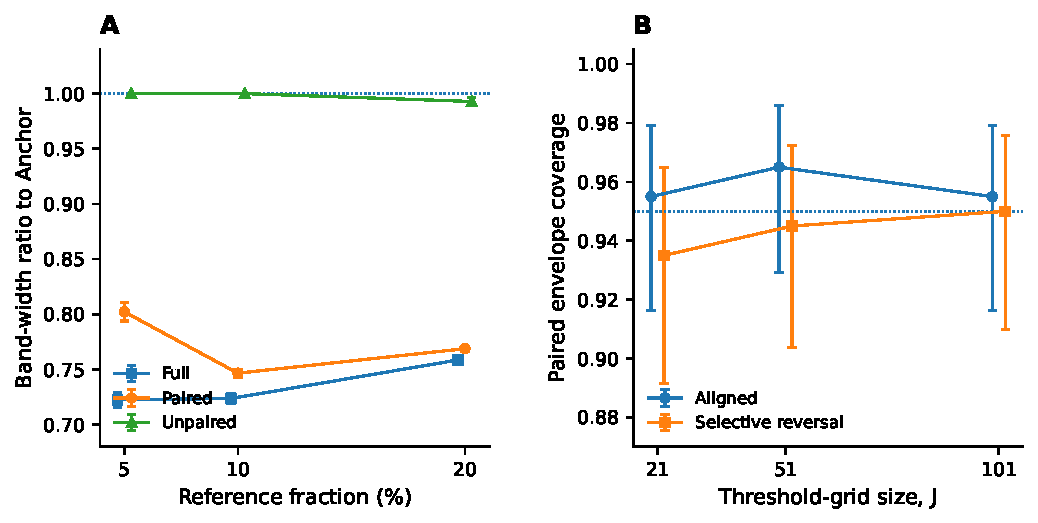
\includegraphics[width=\linewidth]{v3/validation.pdf}
\caption{Pairing and dense-threshold validation. (A) Mean width ratios in the matched ablation, with $\pm1.96$ Monte Carlo standard errors of within-replication ratios, 500 replications per budget. Both certified rules use the same total error budget. (B) Paired monotone-envelope coverage on a common 1,001-point evaluation grid; bars are exact cellwise binomial 95\% intervals. The 200 datasets per mechanism are shared across threshold resolutions.}\label{fig:validation}
\noindent Alt text: Paired retains substantially more width improvement than the unpaired bound. Dense-grid envelope coverage is close to nominal, with visible Monte Carlo uncertainty.
\end{figure}


\subsection{Exact operating characteristics, rotation and numerical checks}
We evaluate the binary experiment of Theorem~\ref{th:boundary} exactly, independent of covariance quadrature. With $p=0.1$, correction amplitude $d=0.2$ and certification error 0.05, we evaluate eight verified counts from 25 to 3,200 and eight associations from $-0.04$ to 0.15; the 192 method--configuration entries are binomial probability sums. Figure~\ref{fig:binary_certification} shows error control and adoption. At zero association, the plug-in harmful-selection probability is 0.444 for $k=50$ and 0.493 for $k=3,200$, the exact binomial rule gives 0.032 and 0.047, and the Hoeffding rule gives approximately 0.008 and 0.007; the largest error among the two lower-bound rules over the evaluated grid is 0.0494. For $\theta=0.04$, exact-binomial adoption rises from 0.100 at $k=50$ to 0.727 at $k=800$ and 0.998 at $k=3,200$, with Hoeffding adoption 0.031, 0.430 and 0.981.

\begin{figure}[htbp]\centering
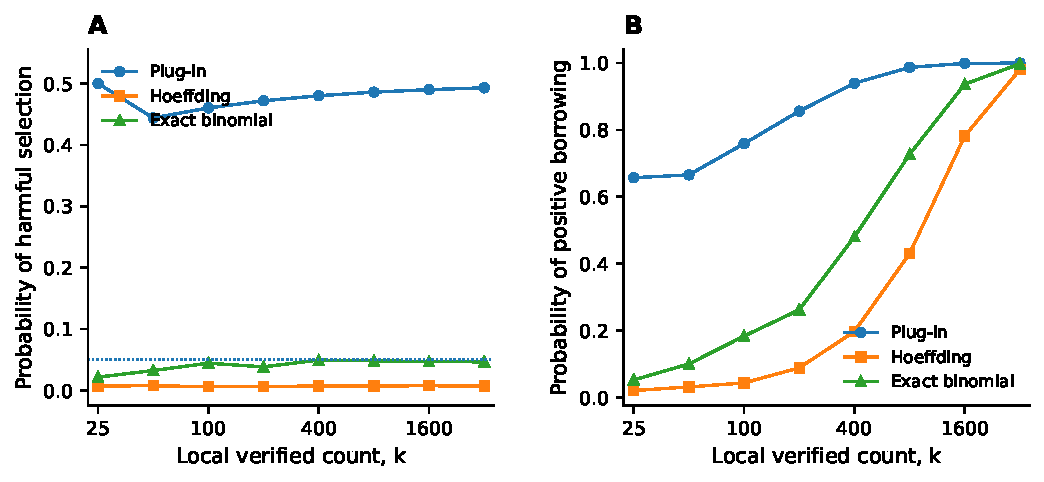
\includegraphics[width=\linewidth]{v2/figure3_binary_certification.pdf}
\caption{Exact binomial operating characteristics of the local submodel, with $p=0.1$, $d=0.2$ and certification error 0.05. (A) Harmful selection at $\theta=0$. (B) Positive borrowing at $\theta=0.04$. All values are exact binomial sums; the two lower-bound rules have distinct power despite controlling error.}\label{fig:binary_certification}
\noindent Alt text: Plug-in harm approaches one half under the null; certified adoption increases with the verified count under a weak positive association.
\end{figure}


We quantify aggregation and numerical accuracy in the remaining experiments. A separate 400-replication experiment uses 200 aligned and 200 reversed datasets with the dependence-valid intersection of three role-specific bands: under alignment, Anchor and Paired cover with frequencies 0.960 and 0.970 and mean widths 0.264 and 0.202, and under reversal both cover with frequency 0.975 and mean width 0.263, while convex endpoint aggregation is wider and covers in every replication. These results concern the explicit construction in Section~S5 and are kept separate from the independent-role primary experiment. All 6,000 primary replications completed without an information fallback. In 60 fitted-data checks, increasing radial directions from 8,192 to 32,768 left every Paired selection unchanged, with largest critical-value change $3.935\times10^{-4}$; the separate Gaussian order-statistic intervals provide the stated Monte Carlo protection. The 6,300 additional design--grid replications use 5,500 distinct datasets because the dense resolutions share samples. Refining radial integration in 30 dense-grid cases changes the selected mesh point in 5 cases, with largest evaluation-width change 3.26\% and largest estimated CDF change 0.0063. All disagreements are retained in Section~S10.

\section{Humidity-specific air-monitor calibration}
\label{sec:application}
\subsection{Scientific question and historical calibration}
Can a mean-calibrated low-cost particle sensor recover the reference instrument's exceedance frequencies, and which discrepancies can a limited reference sample establish? The EPA long-term study collocated six particulate-matter sensor types with reference instruments at seven United States sites \citep{Barkjohn2025}. We use its processed PurpleAir series: 2,814 complete site-days from 22 July 2019 to 1 January 2021, spanning 530 dates and 76 calendar weeks. Date recovery preserves the original observation identifiers and confirms unique site--date combinations, and the target is the processed collocation series with the source quality-control exclusions left unchanged.

We separate historical calibration from subsequent distributional verification. All 985 site-days in 2019 fit the linear correction
\begin{equation}\label{eq:epacal}
 \widetilde S=3.098+0.486S-1.127(X-50)/20,
\end{equation}
where $S$ is uncorrected sensor concentration in micrograms per cubic metre and $X$ is relative humidity in percent. Full-precision coefficients are retained in the code. The remaining 1,829 site-days form the 2020--2021 audit frame. The same historical sample fits the anchor and surrogate distribution regressions, whose predictions and the calibration equation are frozen before reference sampling in the audit frame, so the historical sample costs 985 reference measurements in addition to any subsequent audit budget.

The outcome regressions model $\log(1+Y)$, with $Y$ the reference concentration. The anchor uses humidity terms, and the surrogate candidate additionally uses sensor concentration and its interactions with a fitted scale regression. Concentration thresholds are transformed inside these regressions, while scientific effects and intervals are reported in the original concentration units. Fixed historical training evaluates temporal transport of the correction without refitting on the audit outcomes; the archived whole-series leave-one-site-out diagnostic addresses a different training design and is not pooled with this analysis.

\subsection{The distributional target and complete-frame discrepancies}
For $K_i(r)=K\{(X_i-r)/10\}$, define
\begin{equation}\label{eq:epatarget}
 \Delta_H(t;r)=\frac{\sum_{i\in H}K_i(r)
       \{\ind(Y_i\leq t)-\ind(\widetilde S_i\leq t)\}}
       {\sum_{i\in H}K_i(r)}.
\end{equation}
This is corrected-sensor minus reference exceedance frequency in the humidity neighbourhood, with positive values indicating overstatement. The targets are $r=30\%,50\%,70\%$ with seven inferential thresholds $5,10,15,20,25,30,40$, which describe concentration levels rather than a regulatory classification. The nonzero kernel supports contain 379, 783 and 482 site-days, and the kernel effective sample sizes $(\sum K_i)^2/\sum K_i^2$ are 315.889, 658.420 and 403.199 before reference subsampling.

Table~\ref{tab:epa_science} reports complete-frame calibration. At $30\%$ humidity, the mean corrected-minus-reference concentration difference is $-0.191$ while the 0.90-quantile difference is $-1.612$, and at concentration 15 the corrected and reference exceedance frequencies are $6.068\%$ and $9.307\%$, a difference of $-3.239$ percentage points. At $70\%$ humidity the mean difference is $-0.227$, the 0.90-quantile difference is $+0.471$, and the exceedance discrepancy at 15 is $+1.157$ percentage points. The sign of the average error therefore does not describe the upper tail.

Figure~\ref{fig:epa} displays the complete discrepancy curves. At $30\%$ humidity the discrepancy is positive at low thresholds and negative above the crossing, reaching 18.602 percentage points at concentration 5. The local station mixtures also differ, with Colorado receiving 43.462\% of kernel weight at $30\%$ humidity and 0.793\% at $70\%$. These are conditional distributions of the recorded station--day mixture, so comparisons across humidity do not isolate a causal humidity effect. Complete-frame values describe what all reference measurements establish, and the subsequent experiment measures which statements remain possible when most audit outcomes are hidden.

\begin{figure}[htbp]\centering
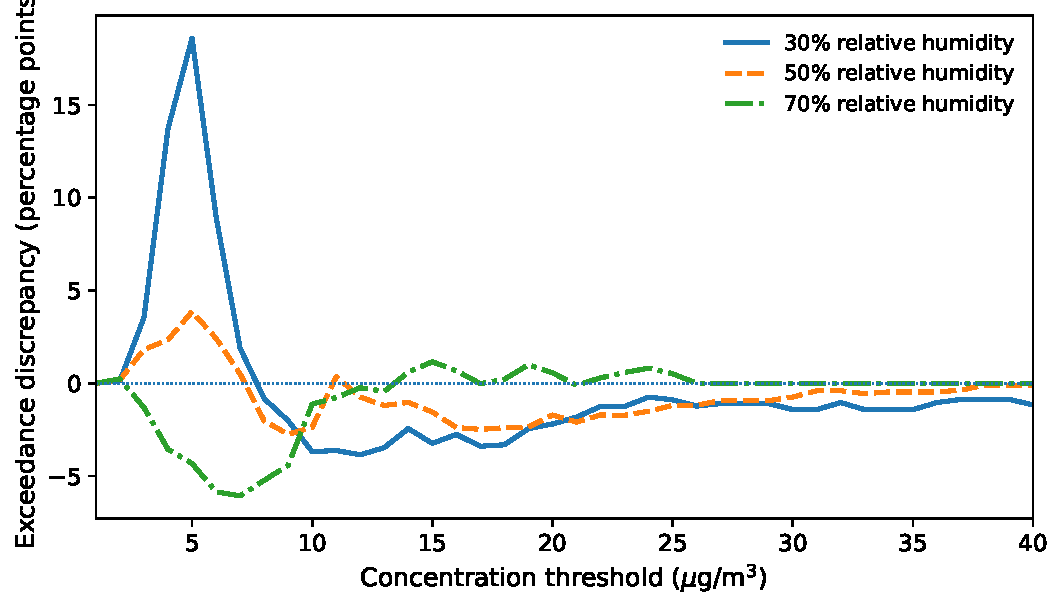
\includegraphics[width=.86\linewidth]{figure2_epa_discrepancy.pdf}
\caption{Complete-frame exceedance discrepancies after historical mean calibration. Positive values indicate overstatement by the corrected sensor. The curves use 40 integer concentration thresholds; inference uses the separately declared seven-threshold grid. These full-reference descriptions have no confidence limits.}\label{fig:epa}
\noindent Alt text: The discrepancy changes sign across concentration thresholds and differs among humidity neighbourhoods.
\end{figure}


\subsection{Designed verification and finite-frame intervals}
We condition on the audit frame and independently randomise gate and evaluation masks, so the uncertainty is design-based for the specified frame. With a unit-specific union probability $p_i$,
\begin{equation}\label{eq:twomasks}
 \pi_{G,i}=p_i/2,\qquad
 \pi_{E,i}=\frac{p_i-\pi_{G,i}}{1-\pi_{G,i}},
\end{equation}
so $\Pr(R_{G,i}\vee R_{E,i}=1)=p_i$. Random auditing uses $p_i=p$ and selective auditing uses the code's bounded sensor-level score normalised to mean $p$, with budgets $p=0.05,0.10,0.20$. Common uniforms nest each role's samples across budgets, all five methods share the same masks, and a unit selected by both roles is measured once. Conditional on the fixed frame, the masks remain independent even though they can overlap.

The evaluation estimate replaces the reference indicators in \eqref{eq:epatarget} by $U_{\lambda,t}$ using $R_E/\pi_E$. With $w_i=K_i/\overline K$, $d_i=m_i-q_i$ and $r_i=(q_i-Z_i,d_i)^\top$, the joint matrix generating its design covariance, scaled by $np$, is
\begin{equation}\label{eq:epacov}
 \Omega_H=\frac pn\sum_{i\in H}w_i^2(\pi_{E,i}^{-1}-1)r_ir_i^\top.
\end{equation}
The gate multiplies each summand by $R_{G,i}/\pi_{G,i}$ to estimate this matrix and uses Bernoulli-design covariance-influence scores for paired calibration; Section~S6 derives the calculation. The corrected-sensor indicators are known throughout the fixed frame and cancel from its randomisation error, which is why the audit uses its own covariance construction rather than the independent-observation formula for consecutive site-days.

Two hundred masks in each of six design--budget cells give 1,200 reference-sampling repetitions. Error budgets are allocated across the three humidity targets for a joint statement over all 21 threshold--humidity combinations, and the common Gaussian enlargement $10^{-8}I$ handles tail-grid singularities without changing point estimates. Complete audit outcomes enter only performance evaluation, and a neighbourhood with fewer than three evaluation references receives a full feasible distribution band that is recorded rather than dropped from coverage.

Supplementary Figure~S1 shows estimates and simultaneous limits from the first retained random-audit mask at the 20\% budget, with 369 unique reference measurements, gate and evaluation counts 31/39, 72/104 and 48/66, and Paired weights 0, 0.8 and 0. Its width at $50\%$ humidity is 15.881 percentage points against 27.632 for Anchor and 14.831 for Full, while at $30\%$ and $70\%$ humidity it retains the anchor and the $70\%$ interval at concentration 10 misses the complete-frame value. Repeated-mask coverage rather than this individual illustration measures calibration.

Table~\ref{tab:epa_budget} compares all five methods, including the two unprotected adaptive selectors. Paired joint coverage is 0.935--0.970 across the six cells, with the 0.935 value carrying Monte Carlo standard error 0.017 and exact binomial intervals retained. Full often produces shorter intervals in this informative-surrogate application: under random auditing its width ratios averaged across humidity are 0.679, 0.667 and 0.660, against 0.985, 0.942 and 0.828 for Paired. Local reference support explains part of this cost. At the 5\% random budget the $30\%$ humidity gate averages 9.93 reference observations and Paired adopts a correction in 1.5\% of masks; at the 20\% budget mean gate support rises to 38.46 and adoption to 40.5\%, while at $50\%$ humidity the counts are 19.67 and 77.37 with adoption rates 10.5\% and 81.5\%. A useful historical correction can therefore remain uncertified in a sparsely monitored neighbourhood, and the mean unique audit budgets are about 91, 183 and 365 measurements on top of the historical 985.

\subsection{Reference budgets and upper-tail precision}
A sign is resolved only when its simultaneous interval excludes zero in the correct direction. At $30\%$ humidity and concentration 5, Paired resolves the positive discrepancy in 1.0\%, 9.5\% and 68.0\% of random masks at budgets 5\%, 10\% and 20\%, against 1.0\%, 8.0\% and 52.0\% for Anchor and 32.0\%, 55.0\% and 89.0\% for Full. At concentration 15 and the 20\% budget, Paired's resolution frequencies are 0\%, 0.5\% and 0\% at the three humidity targets, because the complete-frame discrepancies there are much smaller than at concentration 5. Sparse auditing therefore leaves measurable upper-tail discrepancies unresolved, and the reported probabilities quantify that gap. All 126,000 method--mask--threshold records, including false-sign events, are retained for the full evaluated grid.

\begin{figure}[htbp]\centering
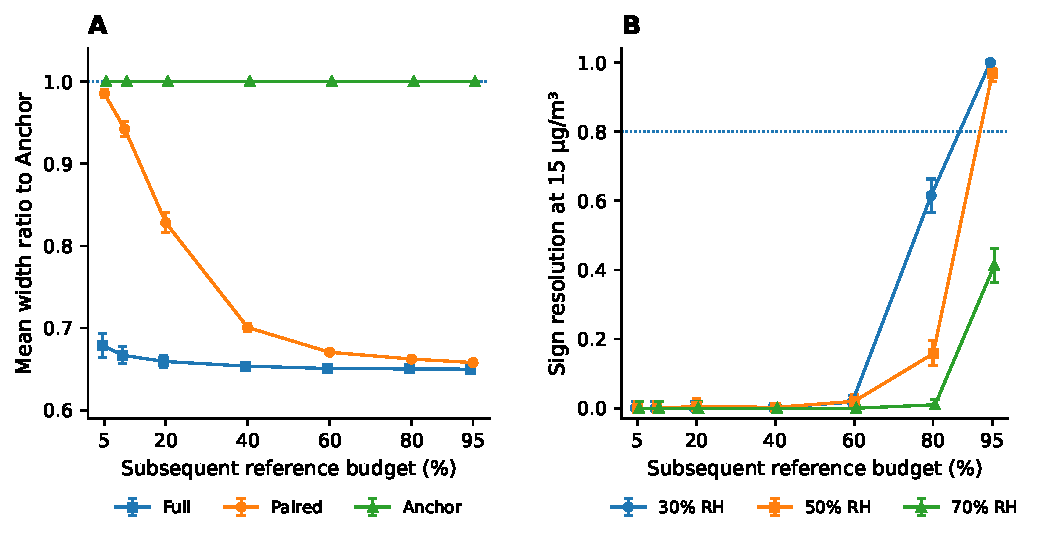
\includegraphics[width=\linewidth]{v3/epa_budget_full.pdf}
\caption{Reference-budget and upper-tail precision under random auditing. (A) Width ratios averaged across humidity within each mask, with $\pm1.96$ Monte Carlo standard errors. (B) Paired's correct sign resolution at concentration 15, with exact binomial 95\% intervals; the dotted line is 0.80. Budgets 5--20\% use the original 200 masks and budgets 40--95\% use 400 masks. Draw families are nested across budgets; historical training costs are additional.}\label{fig:epa_budget}
\noindent Alt text: Increasing reference budgets allows smaller upper-tail differences to be resolved, but the 70-percent humidity discrepancy remains unresolved in many masks even at a 95-percent budget.
\end{figure}


The upper-tail non-resolution motivates a fixed follow-up at budgets 40\%, 60\%, 80\% and 95\% with 400 nested random-audit masks per budget. Historical regressions, thresholds, humidity targets and the selector are unchanged, and all low-budget results are retained. The new experiment contributes 1,600 budget--mask combinations, with four budgets sharing each of 400 independent uniform-draw families. At concentration 15, Paired's sign-resolution probabilities at $p=0.80$ are 0.615, 0.158 and 0.010 for the three humidity targets, and at $p=0.95$ they are 1.000, 0.968 and 0.412, the last with exact 95\% Monte Carlo interval [0.364, 0.462]. Among evaluated subcensus budgets, 95\% is the first to exceed 80\% observed resolution at 30\% and 50\% humidity, and none does so at 70\%; a complete reference census determines the finite-frame contrast exactly as a separate endpoint. Joint coverage over all 21 combinations in the added cells is 0.948--0.975, and Figure~\ref{fig:epa_budget} displays the complete budget trajectory. The 95\% budget uses about 1,737 distinct audit references in addition to the historical 985, so a one-percentage-point upper-tail discrepancy can require nearly complete verification under a familywise raw band even when the sensor correction reduces width. This precision requirement holds for the stated frame and interval shape, and all thresholds, incorrect-sign events and Monte Carlo intervals are retained.

\section{Discussion}
Pairing the candidate and anchor critical values makes the uncertainty of a borrowing gain depend on how much is borrowed. The covariance-set result gives a finite-sample benchmark, the feasible multiplier construction retains the cancellation at the local reference-information scale, and the weak-signal experiment relates the reference information needed to certify a correction to the squared size of its attainable gain.

The matched ablation identifies the contribution of pairing. A small simultaneous gain can be estimable as a difference while separate bounds for its two terms remain too wide, and the dense-grid and non-Gaussian experiments show that this mechanism operates beyond a short threshold vector. Numerical integration and statistical calibration remain separate components of uncertainty. The oracle comparison is made on its stated certification event, and the implemented statistical guarantee is asymptotic; a limitation of the present implementation is that finite-sample coverage in scarce neighbourhoods must be read from the reported simulations rather than from the theorem.

The candidate class sets the remaining limits. Matrix projection can exploit a reversed relationship outside the nonnegative scalar path, and Full can be more efficient under strong alignment; Paired controls whether the fitted correction is used along the proposed path. The complete comparisons report these costs alongside the gains.

In the air-monitoring study, historical mean calibration and subsequent distributional verification answer different questions. A large lower-concentration discrepancy is established with a modest audit, whereas a one-percentage-point upper-tail difference may require nearly complete verification under the same simultaneous family. Designed reference sampling separates this precision requirement from environmental population sampling.

\section*{Data availability}
The EPA analysis table, source-verified date mapping and original computational archive are available in the public repository \url{https://github.com/Stork343/surrogate-assisted-local-conditional-distribution-inference}, source commit \texttt{70c47c512ab485edf502f16914f9ff481cc6be88}. The V3 reproduction package dated 29 September 2026 accompanying this manuscript contains the revised code, all generated results, input checksums and commands for rebuilding its tables and figures. The processed audit population and the historical calibration sample are identified separately.

\section*{Acknowledgements and funding}
This work was partially supported by the Beijing Natural Science Foundation (1242005), the Fundamental Research Funds for the Central Universities and the Research Funds of Renmin University of China (25XNN015), and the Ministry of Education Humanities and Social Sciences Research General Project (25YJA910005).

ChatGPT assisted the methodological revision, mathematical derivations, software development, numerical checks and drafting. Earlier computational development also used OpenAI Codex. These tools are not authors; responsibility for the submitted research, analysis and text rests with the authors.

\section*{Conflict of interest}
The authors declare no conflicts of interest.

\section*{Supplementary material}
The Supplement provides proofs, primitive and growing-grid conditions, numerical calibration details, rotating-role inference, the design-based audit extension and complete numerical results. The reproduction package provides executable code and the input and output data.


\bibliographystyle{plainnat}
\bibliography{references}
\clearpage\begin{table}[p]\centering\setstretch{1.0}
\caption{All six methods at a common sample size and reference fraction.}\label{tab:simulation}
\setlength{\tabcolsep}{3pt}
\begin{tabular}{llrrrr}\toprule
Mechanism & Method & Coverage & Grid ISE & $\Delta$ ISE (MCSE) & Gain \\\midrule
Aligned & Anchor & 0.956 & 3.074 & 0.000 (0.000) & 0.000 \\
 & Full & 0.960 & 1.419 & -1.656 (0.123) & 180.739 \\
 & Trace & 0.962 & 1.420 & -1.654 (0.121) & 180.373 \\
 & Plug-in & 0.962 & 1.427 & -1.647 (0.120) & 179.937 \\
 & Projection & 0.958 & 1.482 & -1.592 (0.121) & 172.550 \\
 & Paired & 0.956 & 1.567 & -1.508 (0.103) & 162.655 \\
\addlinespace[3pt]
Weak & Anchor & 0.960 & 2.899 & 0.000 (0.000) & 0.000 \\
 & Full & 0.966 & 2.526 & -0.373 (0.072) & 31.131 \\
 & Trace & 0.964 & 2.575 & -0.324 (0.058) & 29.995 \\
 & Plug-in & 0.962 & 2.580 & -0.318 (0.056) & 29.746 \\
 & Projection & 0.960 & 2.677 & -0.222 (0.063) & 23.600 \\
 & Paired & 0.960 & 2.899 & 0.000 (0.000) & 0.000 \\
\addlinespace[3pt]
Reversal & Anchor & 0.954 & 3.080 & 0.000 (0.000) & 0.000 \\
 & Full & 0.958 & 3.909 & 0.829 (0.063) & -72.220 \\
 & Trace & 0.954 & 3.080 & 0.000 (0.000) & 0.081 \\
 & Plug-in & 0.954 & 3.080 & 0.000 (0.000) & 0.081 \\
 & Projection & 0.966 & 1.901 & -1.178 (0.106) & 125.115 \\
 & Paired & 0.954 & 3.080 & 0.000 (0.000) & 0.000 \\
\addlinespace[3pt]
No signal & Anchor & 0.968 & 3.000 & 0.000 (0.000) & 0.000 \\
 & Full & 0.968 & 3.006 & 0.007 (0.009) & -0.683 \\
 & Trace & 0.966 & 3.003 & 0.003 (0.004) & -0.217 \\
 & Plug-in & 0.966 & 3.005 & 0.005 (0.005) & -0.232 \\
 & Projection & 0.958 & 3.105 & 0.105 (0.030) & -7.431 \\
 & Paired & 0.968 & 3.000 & 0.000 (0.000) & 0.000 \\
\bottomrule\end{tabular}
\par\raggedright\noindent Each row uses 500 replications with $n=6,000$ and random verification at $p=0.10$. Grid ISE, its mean paired difference from Anchor ($\Delta$ ISE) and mean Gaussian critical-value gain are multiplied by $10^3$. MCSE is the paired-difference Monte Carlo standard error. Negative $\Delta$ ISE and positive gain indicate improvement; Figure~\ref{fig:simulation_comparison} reports widths and harmful-selection frequencies. Supplementary Table~S1 contains all twelve cells and Monte Carlo uncertainties.
\end{table}
\begin{table}[p]\centering\setstretch{1.0}
\caption{Complete-frame calibration after historical training.}\label{tab:epa_science}
\setlength{\tabcolsep}{4pt}
\begin{tabular}{rrrrrr}\toprule
RH (\%) & Local rows & Mean diff. & $Q_{.90}$ diff. & Ref. $>15$ & Sensor $>15$ \\\midrule
30 & 379 & -0.191 & -1.612 & 9.307 & 6.068 \\
50 & 783 & -0.380 & -0.493 & 7.993 & 6.439 \\
70 & 482 & -0.227 & 0.471 & 7.038 & 8.194 \\
\bottomrule\end{tabular}
\par\raggedright\noindent Differences are corrected sensor minus reference in $\mu\mathrm{g}/\mathrm{m}^3$; exceedance frequencies are percentages. The frame has 1,829 site-days and the historical training sample 985. These are complete-frame descriptions.
\end{table}

\end{document}
